% Chapter Template

\chapter{Introduction} % Main chapter title

\label{Chapter2} % Change X to a consecutive number; for referencing this chapter elsewhere, use \ref{ChapterX}

\lhead{Chapter 1. \emph{Introduction}} % Change X to a consecutive number; this is for the header on each page - perhaps a shortened title
\setstretch{2}
%----------------------------------------------------------------------------------------
%	SECTION 1
%----------------------------------------------------------------------------------------

\section{Motivation}

Supersonic combusting ramjet, or scramjet, engines are on the forefront of supersonic transportation development because of their simplicity and promising outlook for steady and reliable supersonic combustion. These engines differ from typical subsonic jet engines, as scramjets have no moving parts and simply rely on shock waves produced at these supersonic speeds to compress the intake air and provide the means for ignition. Shown in Figure \ref{fig:scramjet} is a diagram of a typical scramjet engine.

One challenge facing the production of these engines is producing steady combustion. Much like keeping a match lit in a hurricane, keeping a flame stabilized at supersonic speeds is quite difficult. One proposed method of flame stabilization is a rectangular cavity, as shown in Figure \ref{fig:Cav}. These cavities, are able provide a re-circulation zone with high temperatures and combustion radicals for strong combustion to occur. Many experimental studies have tested the flame-holding abilities of cavities in strong combustion cases \cite{ben2000experimental,ben2001cavity,do2009plasma,yilmaz2013investigation}. Strong combustion occurs when the fuel-air mixture is optimized for efficient fuel burning. The mixture in strong combustion cases occur in proper stoichiometric proportions. These studies focused on cavity dimensions and how the length to depth ratio, L/D, affects key ignition and flame holding characteristics, such as stagnation pressure, stagnation temperature, fuel air mixture, and residence time. Ben-Yakar concluded that with L/D ratios between 4 and 10, strong combustion can be sustained in these cavities for total enthalpy flight conditions of Mach 8, 10, and 13\cite{ben2001cavity}. Also noted in several investigations is the presence of strong acoustic waves\cite{unalmis2004cavity,heller1996letter,williams2007supersonic, mcgregor1970drag,luo2011drag, sato1999advanced}. 

Similar to blowing air over an empty bottle to create a tone, the freestream air traveling over and interacting with these cavities produces acoustic waves. In these cavities, a shear layer develops between the high speed freestream and the slower, re-circulating air in the cavity. As the shear layer travels downstream, it begins to drop. This drop in the shear layer is caused by a pressure gradient present between the freestream and the cavity. When the cavity is long (L/D $>$ 20), there is only a small eddy in the upstream corner of the cavity. The eddy created is not strong enough to keep the shear layer out of the cavity, and thus the shear layer grows into the cavity. In these long cavities, the shear layer can grow to the bottom of the cavity, entraining mass from the cavity. In smaller cavities (L/D $\sim$ 5), the eddy is relatively larger, taking up nearly the entire cavity. This strong eddy inhibits the mass transfer from the cavity to the shear layer, making the shear layer smaller and less likely to grow into the cavity. Also, in these smaller cavities, there is a stronger pressure gradient, making it harder for the shear layer to grow into the cavity. However, due to the unsteady nature of the flow and the pressure gradient, the shear layer can still dip into the cavity. By the time the shear layer reaches the downstream wall of the cavity, it has lowered to a point where the interaction of the shear layer with the downstream wall of the cavity produces strong pressure waves, which propagate upstream, ultimately resonating within the cavity. 

Other experimental studies have investigated the acoustic properties of these cavities \cite{unalmis2004cavity,heller1996letter,williams2007supersonic, mcgregor1970drag,luo2011drag, sato1999advanced}. These investigations concluded that the acoustic waves generated by supersonic cavities produce several undesirable effects. One effect, investigated by McGregor is the induced drag associated with rectangular cavities. The effect of pressure waves within these cavities can increase the drag by as much as 250\% \cite{mcgregor1970drag}. These acoustic waves can also have an adverse effect on equipment and the crew. At low frequencies, the resonating acoustic waves can cause structural damage to the engine. At high frequencies, these waves can cause uneasiness in crew members \cite{mcgregor1970drag}.

Conclusions drawn from these investigations have led to the desire to suppress these acoustic waves. Suppressing these waves would reduce drag on the engine and cause less damage to the engine or the crew. However, stabilizing these acoustic waves could reduce the effectiveness of these cavities because mass transfer and residence time are important to flame holding \cite{ben2001cavity}. These acoustic waves could also have the potential to assist in combustion when conditions for weak combustion are present. Weak combustion, as is studied in this investigation, is at lean fuel air mixture conditions. Sato et al.\cite{sato1999advanced} investigated the enhancement of mixing due to acoustic waves. They concluded that mixing was enhanced by these acoustic waves and the rate of enhancement was controlled by the cavity's shape. However, the investigations performed by Sato et al. did not include the cavity as a flame-holder. The cavity was only used to produce the mixing enhancing acoustic waves. 

One study, though, focused on the ability of cavity-induced acoustic waves to enhance mixing \cite{sato1999advanced}. Their experimental setup, as shown in Figure \ref{fig:sato} shows that the wall-mounted cavities were used exclusively as acoustic wave generators to enhance the mixing of the freestream and the injected gas. Their study showed that the cavity acoustic waves produced had enough energy to enhance mixing. This study will attempt to combine the flame-holding characteristics of these cavities with the acoustic wave assisted mixing. One main difference between Sato's study and this investigation is the location of the enhanced mixing. In this study, the primary focus of studying the acoustic waves is to understand their mixing properties within the flame-holding cavities, rather than outside the cavity. The acoustic waves generated inside the cavity should have nearly the same strength as the waves that escaped the cavity in Sato's study. Because of this, the mixing effects observed in Sato's study should also be present and observable within these flame-holding cavities. 

Few, if any, experimental studies have investigated the acoustic properties of these cavities as they assist in mixing and the enhancement of combustion at lean conditions. This investigation is broken into three parts: acoustic properties of cavities, flame-holding properties of cavities, and initiation and extinction. Together, these provide a clear interpretation of a cavity's suitability as an effective flame holder during weak combustion conditions. It is the goal of the investigation to show that the acoustic waves present in these cavities play a significant role in mixing, providing enhanced mixing in lean conditions to stabilize the reaction until more stable engine conditions are achieved.


\section{Background}

%-----------------------------------
%	SUBSECTION 1
%-----------------------------------
\subsection{Acoustic Properties}

The first part of the investigation isolated the acoustic properties of the cavities. To calculate the frequency inside the cavity, a modification derived from Rossiter's semi-empirical formula, shown in Equation \ref{eq:freqOG}, was used. This relationship is able to incorporate the coupling that exists between the acoustic waves and the vortex shedding\cite{rossiter1964wind}. However, this relationship does not take into consideration the compressibility effects within the cavity. For this investigation, the frequency of a cavity was estimated using an empirical equation derived by Heller and Delfs \cite{heller1996letter}, as shown in Equation \ref{eq:freq}.  Heller and Delfs modified the equation based on their investigation to account for compressibility effects and higher speed of sound within the cavity \cite{ben2001cavity}. The Heller and Delfs equation is estimated to be able to predict the frequency within the cavity $\pm$10\%\cite{heller1996letter}.

\begin{equation}
f_m = \frac{m-\alpha}{\{M_{\infty}+1/k\}} \cdot \frac{U_\infty}{L}
\label{eq:freqOG}
\end{equation}

\begin{equation}
f_m = \frac{m-\alpha}{\{M_{\infty}/\sqrt{1+[(\gamma_{\infty}-1)/2]M_{\infty}^2}+1/k\}} \cdot \frac{U_\infty}{L}
\label{eq:freq}
\end{equation}

Depending on the mode of the strongest acoustic waves, frequencies of these waves will be expected to be between 16.7kHz and 30 kHz for the first mode. It was observed that as L/D increases, the dominant oscillatory mode also increases \cite{ben2001cavity}. However, these base modes should be present within the cavities modeled, but they may not be the strongest modes. For this part of the investigation, three L/D ratios will be investigated: 5, 7, and 9. From the equation, it can be seen that the frequency generated by the cavity is a function of the freestream test gas conditions and length of the cavity. Keeping the freestream conditions nearly identical while changing the length of the cavity will produce different frequencies within the cavity. Data from these tests will lead to the direct comparison of the acoustic properties of the cavities, such as frequency and relative strength, as a function of cavity frequency. Also investigated at each of the L/D ratios was an angled downstream wall to observe the passive suppression of the normally present acoustic waves, as illustrated in Figure \ref{fig:angled}

%-----------------------------------
%	SUBSECTION 2
%-----------------------------------

\subsection{Flame Holding}

The second part of the investigation will be used to isolate the combustion and flame-holding properties of the cavities. As shown by the investigations of Ben-Yakar, L/D ratios between 4 and 10 can sustain strong combustion in these cavities \cite{ben2001cavity}. Because this is a new experiment with a new expansion tube facility, it is important to confirm the flame-holding capabilities of these cavities for the environments that can be achieved. For testing, a strong, stoichiometric, fuel-air mixture will be used and each L/D ratio will be tested, along with its angled downstream wall counterpart. If the cavity model shows promising results of flame-holding, the fuel-air mixture will then be diluted with nitrogen to observe the effects of the acoustic waves as the combustion becomes weaker, which is the third part of this investigation. 

For flame holding to occur, certain conditions must be met within the cavity. One of these conditions is recirculation, as illustrated in Figure \ref{fig:angled}. Recirculation within the cavity allows the fuel and air to slow down and mix to the proper stoichiometric conditions before igniting. The physical parameters of the cavity affect this recirculation. For cavities with a L/D ratio of greater than 10-13 are considered closed cavities, as shown in Figure \ref{fig:Closed}. Closed cavities do not provide sufficient mass transfer between the freestream and the cavity for proper recirculation. The length of the cavity allows for the shear layer to drop within the cavity due to a pressure gradient between the cavity and the freestream, effectively creating two weak eddies within the cavity. These eddies are not strong enough to escape into the freestream. However, cavities with a L/D ratio between 4 and 10 do not experience this significant drop in the shear layer, resulting in one strong eddy within the cavity, as illustrated in Figure \ref{fig:Open}. These cavities are considered open, and are strong enough to provide sufficient mass transfer between the cavity and the freestream, resulting in effective recirculation \cite{ben2000experimental}.Computational investigations by Gruber et al. show that there exists one large vortex near the downstream edge of the cavity and a secondary vortex exists near the upstream wall of an open cavity \cite{gruber2001fundamental}. This downstream vortex, which interacts with the unstable shear layer, controls the mass transfer between the cavity and the freestream gas. This process is illustrated in Figure \ref{fig:vortex}. 

The recirculation of a cavity is characterized by its residence time. The residence time is the amount of time in which the test gas remains within the cavity. For the air-breathing scramjet engines, residence time is particularly important. The fuel and air have less than 1ms to mix and ignite, so any extra time the cavity gives to the mixing and ignition process has the potential to be extremely useful. Previous cavity investigations have shown that cavities can provide residence times on the order of 1ms, effectively doubling the amount of time the fuel and air have to mix and ignite. 

One last feature of the cavities is that they provide a hot anchor point for the flame. The initial step of the cavity causes a shear layer to form, which separates the high velocity freestream from the low velocity mixing flow within the cavity. When the freestream gas slows down in the cavity, the kinetic energy within the flow is converted into mostly thermal energy. This increases the temperature within the cavity, providing a "hot zone," which is hot enough for auto-ignition of the fuel-air mixture. The hot zone provides a point which the flame can latch onto and stabilize itself to continue the combustion process. 


%-----------------------------------
%	SUBSECTION 3
%-----------------------------------

\subsection{Initiation and Extinction}

The third part of the investigation is used to observe the effect that the acoustic waves have on the flame-holding characteristics of the cavities in a non-stoichiometric fuel-air mixture. For these experiments, both flat and angled wall cavities will be tested at the same conditions. Shown by results of the acoustic investigation, the angled walls do suppress the propagating acoustic waves within the cavity, so any observable differences between the results of the angled versus flat downstream wall will be assumed to be due to the cavity acoustics. Ideally, the results of these tests would be to show that the flat downstream wall, and thus the cavity acoustics, do enhance the mixing of the fuel and air, producing stronger combustion than the angled downstream wall. More details about this investigation are included in the Future Works section of this thesis, Chapter \ref{Chapter5}.


%-------------------------------------------------------
%    FIGURES
%------------------------------------------------------
\newpage

\begin{figure}
\centering
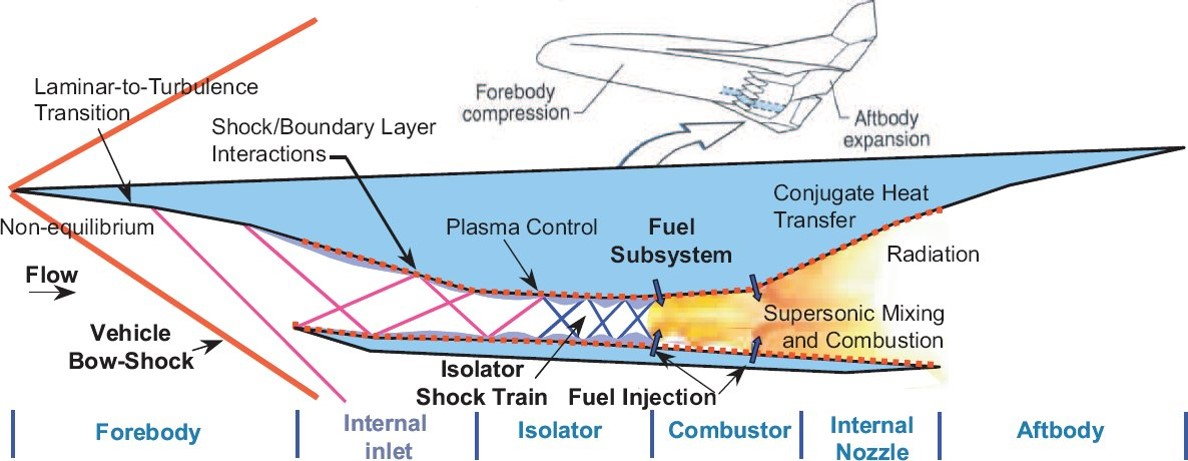
\includegraphics[width=\textwidth]{Figures/scramjet.jpg}
\caption[Scramjet Diagram]{Diagram of a typical scramjet engine, showing shocks produced within the engine. \cite{scramjetFig}}
\label{fig:scramjet}
\end{figure}

\begin{figure}
\centering
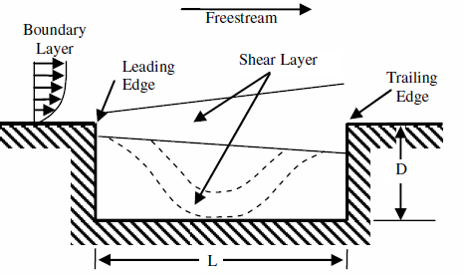
\includegraphics[height=3in]{Figures/CavityDiagram.png}
\caption[Diagram of typical cavity]{Typical hypersonic cavity schematic \cite{lazar2008control}.}
\label{fig:Cav}
\end{figure}

\begin{figure}
\centering
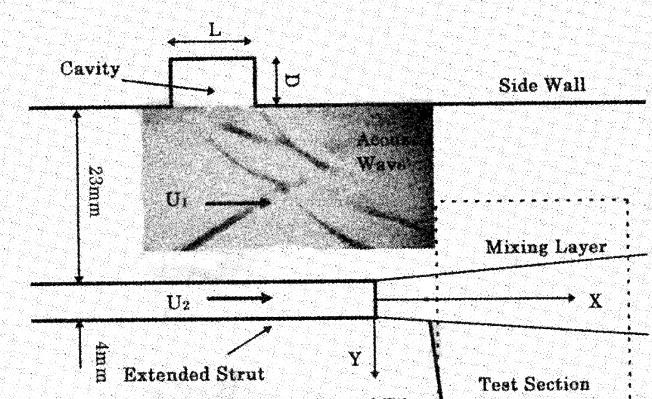
\includegraphics[height=3in]{Figures/CavMix.jpg}
\caption[Cavity-Actuated Mixing]{Mixing enhanced by acoustic waves produced by a side wall-mounted cavity \cite{sato1999advanced}}
\label{fig:sato}
\end{figure}

\begin{figure}
\centering
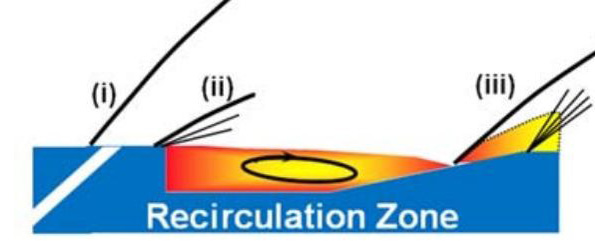
\includegraphics[width = \textwidth]{Figures/Angled.jpg}
\caption[Diagram of typical cavity showing recirculation]{Typical hypersonic cavity schematic showing recirculation and angled downstream wall \cite{do2009plasma}.}
\label{fig:angled}
\end{figure}

\clearpage

\begin{figure}
\centering
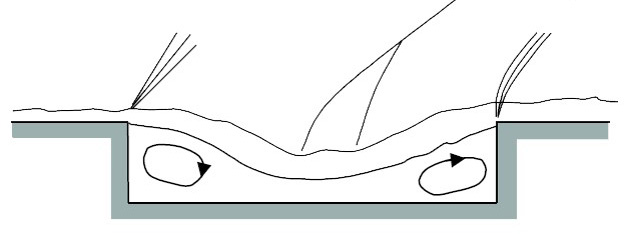
\includegraphics[width = \textwidth]{Figures/ClosedCav.jpg}
\caption[Eddies within a closed cavity]{Eddies within a closed cavity \cite{ben2000experimental}. The shear layer drops into the cavity, creating two separate, weak eddies. The eddies are not strong enough to provide the mass transfer between the cavity and the freestream needed for stable combustion.}
\label{fig:Closed}
\end{figure}

\begin{figure}
\centering
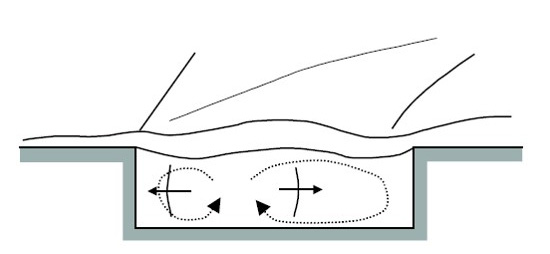
\includegraphics[width=\textwidth]{Figures/OpenCav.jpg}
\caption[Eddies within an open cavity]{Eddies within an open cavity \cite{ben2000experimental}. The eddies formed in an open cavity are strong enough to expel mixed fuel and air into the freestream, allowing stable combustion to occur.}
\label{fig:Open}
\end{figure}


\begin{figure}
\centering
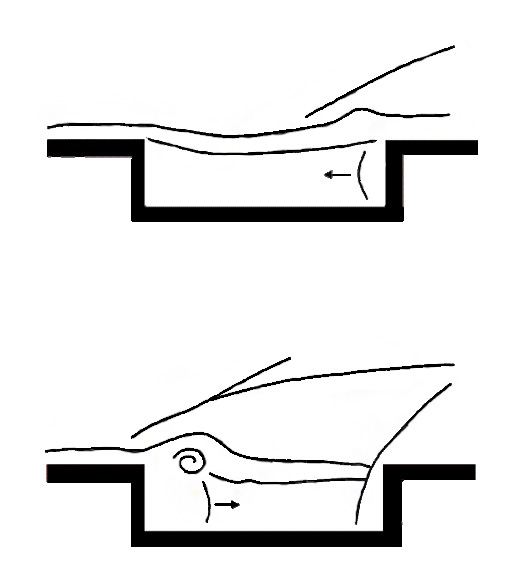
\includegraphics[width=\textwidth]{Figures/SheddingVortices.jpg}
\caption[Shedding vortex process that occurs within cavities]{Shedding votex process that occurs within cavities \cite{ben2000experimental}. Shear layer first interacts with downstream wall, producing a pressure wave that travels upstream (above). These pressure waves interact with the upstream wall and assist in shedding vortices from the leading edge (below).}
\label{fig:vortex}
\end{figure}


